\section{Implementing the Variational Autoencoder (VAE)} \label{p1}

For this problem we will be using \texttt{PyTorch} to implement the variational autoencoder (VAE) and learn a 
probabilistic model of the MNIST dataset of handwritten digits. Formally, we observe a sequence of binary pixels 
$\bx \in {\{0,1\}}^{d}$, and let $\bz \in \Re^{k}$ denote a set of latent variables. Our goal is to learn a 
latent variable model $p_{\theta}(\bx)$ of the high-dimensional data distribution $p_{\text{data}}(\bx)$.

The VAE is a latent variable model that learns a specific parameterization $p_{\theta}(\bx) = \int p_{\theta}(\bx, \bz)d\bz
= \int p(\bz)p_{\theta}(\bx \mid \bz)d\bz$. Specifically, the VAE is defined by the following generative process:

\begin{equation} \label{eq:1}
    p(\bz) = \calN(\bz \mid 0, I)
\end{equation}

\begin{equation} \label{eq:2}
    p_{\theta}(\bx \mid \bz) = \text{Bern}\left(\bx \mid f_{\theta}\left(\bz\right)\right)
\end{equation}

In other words, we assume that the latent variables $\bz$ are sampled from a unit Gaussian distribution 
$\calN(\bx \mid 0,I)$. The latent $\bz$ are then passed through a neural network decoder $f_{\theta}(\cdot)$ to obtain the 
\textit{logits} of the $d$ Bernoulli random variables which model the pixels in each image.

Although we would like to maximize the marginal likelihood $p_{\theta}(\bx)$, computation of $p_{\theta}(\bx) =
\int p(\bz) p_{\theta}(\bx \mid \bz)d\bz$ is generally intractable as it involves integration over all possible values of $\bz$. 
Therefore, we posit a variational approximation to the true posterior and perform amortized inference as we have seen in class:

\begin{equation} \label{eq:3}
    q_{\phi}(\bz \mid \bx) = \calN\left(\bz \mid \mu_{\phi}\left(\bx\right), \text{diag}\left(\sigma_{\phi}^2\left(\bx\right)\right)\right)
\end{equation}

Specifically, we pass each image $\bx$ through a neural network which outputs the mean $\mu_{\phi}$ and diagonal covariance 
$\text{diag}(\sigma_{\phi}^2(\bx))$ of the multivariate Gaussian distribution that approximates the distribution over latent 
variables $\bz$ given $\bx$. We then maximize the lower bound to the marginal log-likelihood to obtain an expression known as 
the \textbf{evidence lower bound (ELBO)}:

\begin{equation} \label{eq:4}
    \log p_{\theta}(\bx) \ge \text{ELBO}(\bx; \theta, \phi) = \E_{q_{\phi}(\bz \mid \bx)} [\log p_{\theta}(\bx \mid \bz) - \KL\left(q_{\phi}\left(\bz \mid \bx\right) \mid\mid p\left(\bz\right)\right)]
\end{equation}

Notice that the negatation of the ELBO decomposes into two terms: (1) \textbf{the reconstruction loss}: $- \E_{q_{\phi}(\bz \mid \bx)}[\log p_{\theta}(\bx \mid \bz)]$, and 
(2) \textbf{the Kullback-Leibler (KL) term}: $\KL (q_{\phi}(\bz \mid \bx) \mid\mid p(\bz))$, e.g. -ELBO = recon. loss + KL div. Hence,
VAE learning objective is to minimize the negative ELBO.

\textbf{How does this relate to Lecture's ELBO?} In lecture, we learned that ELBO objective as 
\begin{center}
    $\log p(\bx; \theta) \ge \sum_{z}q(\bz; \phi) \log p(\bz, \bx; \theta) + H(q(\bz; \phi)) = \calL(\bx; \theta, \phi)$ \\
    $\log p(\bx; \theta) = \calL(\bx; \theta, \phi) + \KL(q(\bz; \phi) \mid\mid p(\bz \mid \bx; \theta))$
\end{center}

where $\theta$ is the decoder, $\phi$ is the encoder. However it is not scalable to define an encoder $\phi$ for each data point $x$,
which is why we introduce the amortized distribution $q_{\phi}(\bz \mid \bx)$ which learns a neural network to regressively provide $\phi$
given $\bx$. If you were to replace $q(\bz; \phi)$ with the amortized function, you will generate the ELBO expression defined above. The problem statements
representation of the ELBO allows you to easily see that maximizing the ELBO really implies minimizing the KL Divergence between $q_{\phi}$ and $p(\bz)$
which means that is has an inclination to train the encoder to make $q$ similar to the prior, serving as a regularization force.  

Your objective is to implement the variational autoencoder by modifying \texttt{utils.py} and \texttt{vae.py}.

\begin{enumerate}[label=(\alph*)]
    \item \points{1a} Implement the reparameterization trick in the function \texttt{sample\_gaussian} of \texttt{utils.py}. 
    Specifically, your answer will take in the mean \texttt{m} and variance \texttt{v} of the Gaussian distribution 
    $q_{\phi}(\bz \mid \bx)$ and return a sample $\bz \sim q_{\phi}(\bz \mid \bx)$.

    \item \points{1b} Next, implement \texttt{negative\_elbo\_bound} in the file \texttt{vae.py}. Several of the functions in \texttt{utils.py} 
    will be helpful, so please check what is provided. Note that we ask for the \textit{negative} ELBO, as \texttt{PyTorch} optimizers 
    \textit{minimize} the loss function. Additionally, since we are computing the negative ELBO over a mini-batch of data 
    ${\{\bx^{(i)}\}}_{i=1}^{n}$, make sure to compute the \textit{average} $- \frac{1}{n}\sum_{i=1}^{n} \text{ELBO}(\bx^{(i)}; \theta, \phi)$ 
    over the mini-batch. Finally, note that the ELBO itself cannot be computed exactly since exact computation of the reconstruction 
    term is intractable. Instead we ask that you estimate the reconstruction term via Monte Carlo sampling

    \begin{equation} \label{eq:5}
        - \E_{q_{\phi}(\bz \mid \bx)} [\log p_{\theta}(\bx \mid \bz)] \approx - \log p_{\theta}(\bx \mid \bz^{(1)})
    \end{equation}

    where $\bz^{(1)} \sim q_{\phi}(\bz \mid \bx)$ denotes a single sample. The function \texttt{kl\_normal} in \texttt{utils.py} 
    will be helpful.
    
    \textbf{Note}: \texttt{negative\_elbo\_bound} also expects you to return the \textit{average} reconstruction loss 
    and \textit{average} KL divergence.

    \item \points{1c} To train the VAE, run
    
    \begin{verbatim}
        python main.py --model vae --train
    \end{verbatim}

    To use GPU acceleration run the command below.
    \begin{verbatim}
        python main.py --model vae --train --device gpu
    \end{verbatim}
    
    Once the run is complete (20000 iterations), it will output (assuming your implementation is correct): the (1) average negative ELBO, (2) average KL term, and (3) average reconstruction loss 
    as evaluated on a test subset that we have selected. These three numbers will be reported to \texttt{submission/VAE.pkl}. To check the accuracy of your values run
    \begin{verbatim}
        python grader.py 1c-0-basic
    \end{verbatim}

    Since we’re using stochastic optimization, you may wish to run the model multiple times and report each metric’s mean and corresponding standard error. We recommend running
    training 5-10 times.
    
    \textbf{Hint}: the negative ELBO on the test subset should be somewhere around 100. If you generate other NELBO values outside this range, please
    revisit your implementation of functions in \texttt{utils.py}, specifically \texttt{sample\_gaussian}.

    Also, to visualize 200 digits sampled from $p_{\theta}(\bx)$, you can run after training:
    \begin{verbatim}
        python main.py --model vae
    \end{verbatim}  

    Your samples will be saved to: \texttt{model=vae\_z=10\_run=0000.png}. The generated samples should look like the image below:

    \begin{figure}[h]
        \centering
        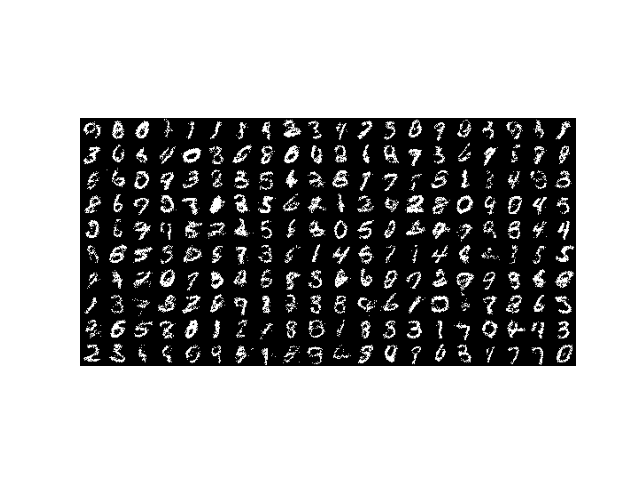
\includegraphics[width=0.8\textwidth]{./figures/vae_gen}
    \end{figure}

    \item \input{01-vae/01-betavae}

\end{enumerate}